\section{Compiler Overview}
Figure \ref{Fig:CompilerStructure} shows the high level structure of Treebeard. The input to the compiler is a JSON file that describes the decision forest model and a set of options. The output of the compiler is a callable function that takes an array of rows and returns an array containing the model's prediction for each row. \TODO{Add a diagram, including IR stages}. The specified set of options includes information such as the batch size, the type of the input features, the type for node thresholds and the type for feature indices \TODO{There are also several optimization related inputs like tile size, type of tiling, pipeline depth etc. Should we mention those?}. Treebeard is written as a dialect in the MLIR framework \cite{MLIR}. At a high level, Treebeard first performs transformations on the trees in the model and subsequently generates and performs optimizations on a more traditional loop based IR. From an implementation perspective, Treebeard first constructs a high level representation of the decision forest inference operation and then progressively optimizes and lowers it to LLVM IR \cite{LLVM}. LLVM is then used to JIT compile the generated IR to executable code. The following sections describe each level of the IR and their lowering in more detail.

\begin{figure}
  \centering
  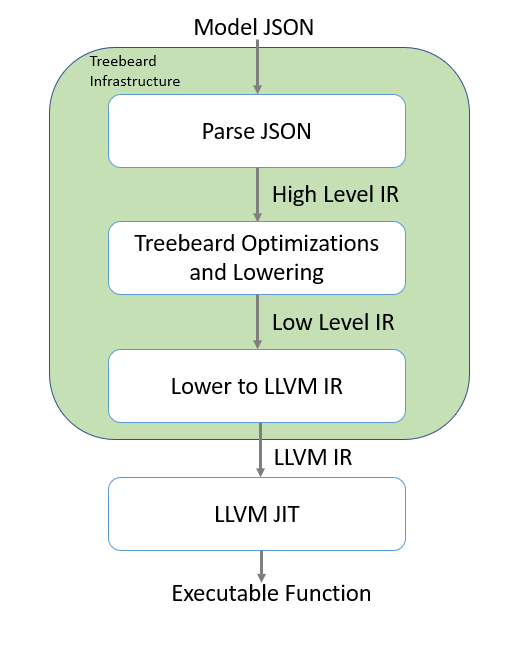
\includegraphics[scale = 0.3]{figures/CompilerStructure.PNG}
  \caption{Treebeard Compiler Structure}
  \label{Fig:CompilerStructure}
\end{figure}

\TODO{Should we describe the dialect's type system?}

\subsection{High Level IR}
Treebeard parses the input JSON file and generates a function with a single MLIR operation, \texttt{predictForest} that represents inference using the input model on a set of rows. The operation contains within it a tree based representation of the model that can be manipulated by optimizing transformations. Transformations on the model such as tiling, tree reordering and leaf padding are done at this level. The structure of the loop nest to walk the iteration space of trees and inputs is also decided at this level of the IR. \TODO{Should we mention that there is a scheduling language to decide this?}

\begin{lstlisting}[language=C++]
func Predict(float rows[batchSize]) {
  predictions = predictForest(rows) 
  return rows
}
\end{lstlisting}

\subsection{Mid Level IR}
The Mid Level IR makes the loop structures and tree walks more explicit. Firstly, the order in which the iteration space of trees and inputs is walked is explicitly specified in the IR through loop nests. Also, tree specific operations such as \texttt{isLeaf}, \texttt{traverseTile}, \texttt{getLeafValue} are introduced so that the traversal of trees explicitly represented. The following listing shows the IR for inference using a model with four trees on an input batch with two rows. The listed IR walks all trees for one input row before moving to the next row. One important point to note here is that details such as the data structure used for the trees are not explicitly encoded in the IR. This allows us to reuse optimization and lowering passes on this level of the IR regardless of what the final in memory representation of the model is.

\begin{lstlisting}[language=C++]
  // Constant that represents the model being compiled
  forest = ensemble(...)
  for i = 0 to 2 step 1 {
    prediction = 0
    for t = 0 to 4 step 1 {
      tree = getTree(forest, t) 
      node = getRoot(tree)
      while (isLeaf(tree, n)==false)  do {
        node = traverseTreeTile(tree, node, rows[i])
      }
      treePrediction = getLeafValue(tree, node)
      prediction = prediction + treePrediction
    }
    predictions[i] = prediction
  }
\end{lstlisting}

The IR listed above is a simplification of the actual IR. The actual IR is strongly typed and in SSA form.

\subsection{Low Level IR}
The IR is finally lowered to a form where the in memory representation of the model is made explicit. Buffers to hold the model values are inserted into the generated code and all tree operations in the mid-level IR are lowered to explicitly reference these buffers. The semantics of all operations are made explicit. For example, \texttt{traverseTreeTile} is lowered into a series of operations to load thresholds, feature indices and features, compare the features with the thresholds and compute the next node to evaluate. This IR is then lowered directly to LLVM IR and JITted.

